\documentclass[iop]{emulateapj}

\usepackage{amsmath}
\usepackage{graphicx}
%\usepackage{fullpage}
%\usepackage{multicol}
%\usepackage{natbib}
%\usepackage{amssymb}
%\usepackage{savesym}
%\usepackage{cancel}
%\usepackage{color}
%\usepackage{caption}
%\usepackage{subcaption}
%\usepackage{tabularx}
%\usepackage{mathtools}
\usepackage{enumitem}
%\usepackage[font=small, labelfont=bf, labelsep=period, justification=justified]{caption}
%\usepackage{afterpage}
%\usepackage{hyperref}

%\usepackage{tikz}
%\def\checkmark{\tikz\fill[scale=0.4](0,.35) -- (.25,0) -- (1,.7) -- (.25,.15) -- cycle;}

%\bibliographystyle{unsrt}
%\setcitestyle{square}

%\providecommand{\e}[1]{\ensuremath{\times 10^{#1}}}
\newcommand{\e}[1]{\ensuremath{\times 10^{#1}}}

%\numberwithin{equation}{section}

\usepackage[T1]{fontenc}

\shorttitle{}
\shortauthors{Matthew Young}

\begin{document}

\title{A Cryogenic Testing Environment for SPT-3G, the Next Generation South Pole Telescope Receiver}
\author{Matthew Young}
\affil{Astronomy \& Astrophysics Department, University of Toronto, ON}
\author{Supervised by: Keith Vanderlinde and Tyler Natoli}
\affil{50 St. George Street\\Toronto, Ontario, Canada\\M5S 3H4}
%\email{young@astro.utoronto.ca}

\begin{abstract}
The next generation optical system for the South Pole Telescope, \textsc{spt-3g}, is set to be deployed in early 2016.  This report outlines the fundamental science goals and operation behind \textsc{spt-3g}, and covers the development of a cryogenic testing environment at the University of Toronto for characterizing the next generation of detectors.  A helium pulse tube driven cryostat housing an adiabatic demagnetization refrigerator has enabled sub-Kelvin temperatures on the \textsc{spt-3g} wafer stage, essential for operating the superconducting detectors.  This has lead to the successful biasing of detectors and verification of the entire integrated readout chain.
\end{abstract}

%\keywords{key,words}


\section{Introduction}

The South Pole Telescope (SPT) is a 10 metre microwave telescope, located at the geographic South Pole in Antarctica.  Designed to observe temperature and polarization anisotropies in the Cosmic Microwave Background (CMB) \citep{spt_collaboration_south_2004}, the telescope has been optimized to operate in the millimetre (mm) band spanning from 75~GHz to 240~GHz.
The next generation optical system to be installed at the beginning of 2016, \textsc{spt-3g}, is to contain over 16,000 polarization sensitive detectors in the focal plane array.  This order of magnitude increase in the number of detectors over the current receiver will allow for high signal-to-noise mapping of both the \textit{E}-mode and \textit{B}-mode CMB polarization anisotropies \citep{benson_spt-3g:_2014}. With the increased sensitivity achieved by \textsc{spt-3g}, significant advances can be made in the fields of large scale structure formation, particle physics, and cosmic inflation.


The \textsc{spt-3g} detector wafers are currently being fabricated by Argonne National Laboratory, using a range of designs to tweak device parameters.  Each wafer is tested within the SPT collaboration, providing characteristic feedback to the nanofabrication process.  The detectors operate in the superconducting transition region for titanium, requiring sub-kelvin cryogenic environments for detector testing.  This report outlines the development of such a system at the University of Toronto (UofT), to assist in the testing and characterization of \textsc{spt-3g} wafers.  This system also features the \textsc{spt-3g} Digital Frequency Multiplexing (DfMUX) readout system, enabling testing of the entire \textsc{spt-3g} detector readout chain at UofT.
In Section~\ref{science_section}, the science goals of \textsc{spt-3g} are outlined, with the instrumentation required to achieve these goals covered in Section~\ref{instrumentation_section}.  Section~\ref{testing_section} details the development of the cryogenic testing facility at UofT, with testing results in Section~\ref{results_section}.  Finally, Section~\ref{data_section} takes a brief look at the processing of \textsc{spt-pol} detector timestreams into usable scientific data.



\section{\textsc{spt-3g} Science Goals}
\label{science_section}

The telescopes location at the Amundsen-Scott South Pole Station provides one of best sites on Earth for observing mm-wavelength anisotropies.  This is in part due to the South Pole's elevation of 2.8~kilometres above sea level, resulting in desirably low levels of atmospheric fluctuation power.  The near zero air humidity also weakens the strong absorption and emission features of atmospheric water vapour at mm-wavelengths.
The current optical design produces a beamwidth of $\sim$1 arcmin at 150~GHz, allowing for high resolution mapping of small-scale CMB features.  Coupled with the high raw sensitivity achievable through the new multi-chroic polarization-sensitive pixel design, \textsc{spt-3g} will be able to extract a wealth of previously unobtainable cosmological information from the CMB.

Lensing measurements of the CMB are capable of probing matter fluctuations out to the last scattering surface, providing a detailed lensing power spectrum.  \textsc{spt-3g}'s precise measurement of the growth of structure on small angular scales places tight constraints on the number of relativistic species at recombination.  Combined with measurements from the \textit{Planck} experiment, it is expected that the sum of neutrino masses will be constrained to within $\sigma(\Sigma m_{\nu})\sim0.06$~eV \citep{benson_spt-3g:_2014}.

Currently pursued by a number of other experiments is the measurement of the energy scale of inflation, described by the tensor-to-scalar ratio \textit{r} of primordial perturbations \citep{samtleben_cosmic_2007}.  While instruments such as \textsc{bicep2}/\textsc{keck} are optimized for measuring low angular modes, they have little or no sensitivity to small-scale temperature and polarization anisotropies.  In order to fully characterize the inflationary and lensing \textit{B}-mode signals, it is vital to take a high-resolution, multifrequency approach.  \textsc{spt-3g} will be capable of producing a high signal-to-noise map of the lensed \textit{B}-modes, achieving a noise level of $\sim3.5\mu$K-arcmin.  When used in conjunction with its exquisite \textit{E}-mode measurements, the lensing potential can be reconstructed, allowing for the separation of the lensing \textit{B}-mode signal from the inflationary signal.  This process is known as "delensing", improving the shape of the tensor power spectrum and constraining \textit{r} to within $\sigma(r)\ll0.01$ \citep{benson_spt-3g:_2014}.

The high angular resolution of the telescope also provides a unique way of probing the largest gravitationally bound objects in the universe, clusters of galaxies.  CMB photons collide with high energy electrons contained within galaxy clusters, where they inverse Compton scatter to higher energies.  This produces a distortion in the CMB signal, known as the Sunyaev-Zel'dovich (SZ) effect.  This effect is largely redshift independent, allowing for the identification of almost every massive cluster above a given mass threshold, depending on instrument sensitivity.  \textsc{spt-3g} will be surveying a nearly identical 2500 deg$^2$ area to \textsc{spt-sz}, albeit with noise levels $\sim$12, 7, and 20 times lower at 95, 150, and 220~GHz, respectively.  The lowering of the cluster mass threshold and extension of redshift reach will allow \textsc{spt-3g} to find $\sim$5000 clusters at a signal-to-noise > 4.5, an order of magnitude more clusters than \textsc{spt-sz}.  The projected \textsc{spt-3g} cluster sample is shown in Figure~\ref{sptsz}.  Complimenting and calibrating the Dark Energy Survey (\textsc{des}) cluster survey, the SZ data is predicted to result in a dark energy figure-of-merit of $\sim$100.

\begin{figure}
	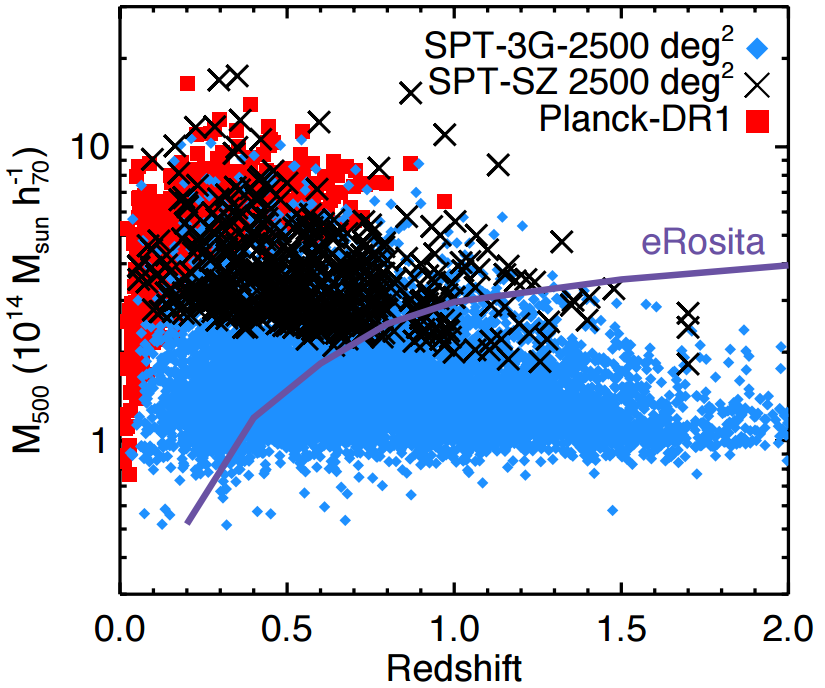
\includegraphics[width=\linewidth]{sz_clusters}
	\centering
	\caption{Mass versus redshift for the SZ clusters discovered by \textsc{spt-sz}, the \textit{Planck} survey, and the projected \textsc{spt-3g} cluster sample.  The increased sensitivity of \textsc{spt-3g} lowers the mass threshold and extends redshift reach, predicting for 5000 newly identified galaxy clusters.  Overplotted is the expected selection threshold for the eRosita X-ray cluster survey \citep{benson_spt-3g:_2014}.}
	\label{sptsz}
\end{figure}

%Measurements produced by \textsc{spt-3g} will impact a range of cosmological fields, including inflationary theories, large-scale structure, and high-energy physics \citep{benson_spt-3g:_2014}.  The search for primordial \textit{B}-modes places constraints on the ratio of power in tensor perturbations to scalar perturbations, tied to the energy scale of inflation \citep{samtleben_cosmic_2007}.  Collected data will also be able to constrain the sum of neutrino masses, using information in the \textit{BB} lensed power spectrum to reduce the upper mass limit down to $\sim$0.06~eV, as well as addressing the neutrino mass hierarchy \citep{benson_spt-3g:_2014}.


\section{\textsc{spt-3g} Instrumentation}
\label{instrumentation_section}

The SPT third-generation receiver design is to also include an improved optical system and cryostat, however this report will focus on the detectors contained in the focal plane array and its novel readout system.

\subsection{Focal Plane Array}

A significant contribution to \textsc{spt-3g}'s leap forward in sensitivity can be attributed to the newly designed focal plane array, featuring 2710 independent pixels compared to \textsc{spt-pol}'s 768.  Each pixel is polarization sensitive across three observing bands at 95, 150, and 220~GHz.  Using a sinuous log-periodic antenna, each pixel can absorb a wide band of mm-wave photons at orthogonal polarizations.  Once absorbed, microstrip transition line filters route the power from each band to one of six independent transition edge sensor (TES) bolometers (one for each band and polarization).   This design results in over 16,000 detectors across the entire focal plane array.  The focal plane array itself consist of 10 nanofabricated 6" wafers, each containing 217 of these polarization sensitive tri-chroic pixels in both left and right-handed configurations (to account for polarization wobble induced by the antenna shape).

\begin{figure}
	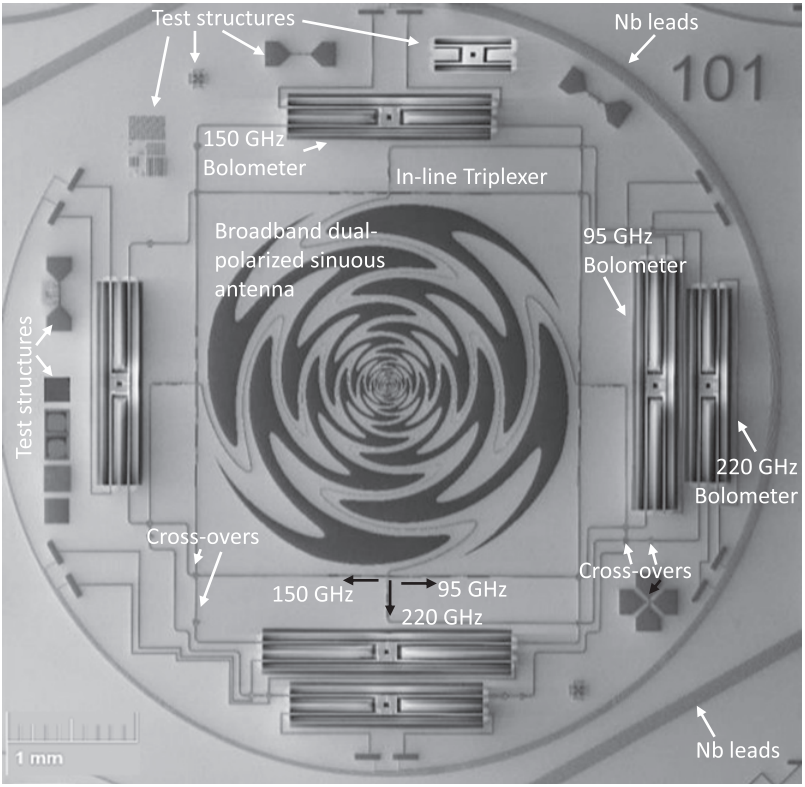
\includegraphics[width=\linewidth]{pixel}
	\centering
	\caption{\textsc{spt-3g} tri-chroic pixel design, featuring a sinuous log-periodic antenna with dual-polarization.  The polarized signal is split into three bands at 95, 150, and 220~GHz, with each band sent to an independent TES bolometer \citep{posada_fabrication_2015}.}
	\label{sptpixel}
\end{figure}

Each detector is essentially a microstrip termination resistor located on a thermally isolated TES bolometer island.  The TES bolometer itself is held in its superconducting phase transition, where a small increase in temperature results in a dramatic increase in resistance.  By passing current through the TES, a change in resistance can be measured after an absorbed photon transmits its energy to the island through the microstrip.  This configuration results in a negative feedback loop, where the increase in resistance restricts the bias current.  This lowers the power passing through the TES, dropping the detector back into its superconducting phase transition.  The bolometer time constant for this process is $\sim$3~ms.

%Each \textsc{spt-3g} wafer fabricated by Argonne National Laboratory contains 217 pixels, with each pixel featuring a sinuous log-periodic antenna, microstrip inductor-capacitor (LC) filters, and six transition edge superconducting (TES) bolometers \citep{benson_spt-3g:_2014}.  A photograph of the pixel design is shown in Figure.  The bolometers are responsible for detecting photons at band centres of either 95~GHz, 150~GHz, or 220~GHz for a given polarization, following the isolation of each signal by the LC filters.  As the TES bolometers are maintained in a superconducting phase transition through electro-thermal feedback \citep{benson_spt-3g:_2014}, a small increase in temperature due to the incident photons will result in a large change in resistivity.

\subsection{Readout System}

If each bolometer within the focal plane array were read out using independent wire pairs, the resulting thermal load would make it near impossible to maintain the array below the TES superconducting transition temperature.  As such, a Digital Frequency Multiplexing (DfMUX) readout system is utilised, allowing 64 bolometers to be read out using a single pair of wires.  Developed by McGill University, the DfMUX system relies on each resistive bolometer being placed in series with a unique inductance \textit{L} and capacitance \textit{C}.  This configuration forms an $LCR_{bolo}$ resonator, allowing the bolometer to be interrogated using a unique resonant frequency.  Recent improvements in the DfMUX bandwidth now permits 64 of these $LCR_{bolo}$ resonators to be placed in parallel, up from 16, with resonances spaced from 1.6 to 4.6~GHz.  A sinusoidal voltage bias can then be fed in on a single pair of wires, consisting of every bolometer's resonant frequency summed together into a single waveform (referred to as a \textit{comb of carriers}) \citep{bender_digital_2014}.  Changes in bolometer resistance from absorbed photons modulates each carrier, appearing as sidebands in the current.  This resulting signal is then amplified using Superconducting Quantum Interference Device (SQUID) amplifiers.

SQUIDs are used as the first amplification stage due to their high gain, low input-impedance, and low noise performance.  The amplifiers consist of a superconducting loop containing two Josephson junctions for allowing the current to be measured.  Any applied magnetic flux to the SQUID will produce a screening current, requiring that the flux within the loop remains at an integer number of magnetic flux quanta.  This results in a periodic voltage output as a function of the magnetic flux in the input coil.  The DfMUX operation requires SQUIDs to first be tuned to the region of maximum gain and linearity, by applying known current flux biases to the input coil \citep{bender_digital_2014}.  The dynamic range of the SQUIDs is capable of limiting the multiplexing factor, and so an inverted copy of the carrier comb in injected prior to the SQUID input coil (referred to as the \textit{nuller}).  The improved DfMUX multiplexing factor of 64 is realised through the use of Digital Active Nulling (DAN), an active feedback loop that nulls both the carriers and sidebands for each bolometer.  Following the DAN stage, the signal is demodulated back to baseband allowing the current from each bolometer to be measured.


%Reading out the thermal loading of each bolometer individually introduces an unnecessary number of wires to the sub-Kelvin stage, and as such, \textsc{spt-3g} utilizes a frequency multiplexing readout system, enabling 64 bolometers to be addressed using a single wire \citep{dobbs_frequency_2012}.  By placing each resistive bolometer in series with a unique LC filter, an LCR resonator is formed \citep{henning_feedhorn-coupled_2012} that can be interrogated using its characteristic resonant frequency, allowing the warm electronics to perform readout in Fourier space.  A digital frequency multiplexing (DfMUX) \citep{dobbs_frequency_2012} system has been developed by McGill University, designed to deliver small amplitude excitations to each resonator with active digital feedback for nulling the subsequent signal.  The error in signal cancellation is then sensitively measured using superconducting quantum interference devices (SQUIDs) \citep{dobbs_frequency_2012}, inferring changes in the bolometer impedance and hence thermal loading.

\section{Testing Environment}
\label{testing_section}

The operation of \textsc{spt-3g} wafers and readout demands sub-Kelvin temperatures, requiring a cryogenic testbed.  The Long Wavelength Lab (LWlab) at UofT currently houses an Olympus 104 cryostat, designed and fabricated by \textit{High Precision Devices} (HPD) in Colorado.  The cryostat consists of several stages, with successively colder and smaller stages located within one another.  The largest of these, a 50~K stage and 3~K stage, are driven by a PT415 helium pulse tube refrigerator developed by \textit{Cryomech}.  This refrigerator relies on the acoustic resonance of sharply pulsed highly-pressurised helium gas.  Pulses travelling through the tube, tuned to a particular resonance, produce heating on one end and cooling temperatures as low as 2~K at the other.  The sub-Kelvin temperatures required for testing \textsc{spt-3g} wafers are then realised using an Adiabatic Demagnetization Refrigerator (ADR) based on the 3~K stage.  

The ADR itself consists of two paramagnetic salt pills, situated within a powerful superconducting electromagnet ($L\sim10$~H).  When a large current is applied to the electromagnet, the produced magnetic field aligns the magnetic domains within the paramagnetic salt pills.  This freezes out a thermal degree of freedom within the salt pills.  Once soaked, removing the current from the coil allows the magnetic domains to realign, reintroducing the thermal degree of freedom.  In accordance with the conservation of energy, this adiabatic realignment process lowers the temperature of the paramagnetic salt pills.  The ADR system installed in the Olympus 104 cryostat features two salt pills, one of Ammonium Iron(III) Sulfate (FAA) and one of Gadolonium Gallium Garnet (GGG), with base temperatures 35~mK and 500~mK respectively.  The FAA pill drives what is referred to as the \textit{ultra-cold stage}, while the GGG pill drives the \textit{itermediate stage}.  The inclusion of an intermediate stage allows the ultra-cold stage to be buffered by the GGG pill's greater cooling power.  This configuration ensures most of the thermal loading from the cold wiring is absorbed at the GGG pill, rather than the FAA.  

The ADR's superconducting electromagnet contains $\sim$5~km of Niobium-Titanium (NbTi) wire looped around the magnet bore.  This NbTi wire is superconducting below $T_c=9.2$~K, resulting in a series resistance of $\sim$0.1~$\Omega$ below the critical temperature.  While superconducting, the NbTi wire has a critical current density of $J_c=10^3$~A$\cdot$mm$^{-2}$ beyond which the superconducting state will break down.  This sets a magnet current upper limit of 19.0~A for this given implementation.  By exceeding this current or the critical temperature $T_c$, the superconductivity of the wire will cease, resulting in the dumping of the magnet's field energy to the 3~K stage.  This scenario is called a magnet "quench", and can cause significant damage to the system.  As such, multiple safeguards have been implemented in both hardware and software to avoid such a scenario.

Following demagnetization, the ADR's ultra-cold temperature is regulated at a chosen setpoint using a Proportional-Integral-Derivative (PID) feedback loop control system.  Thermometry feeds in the stage temperature to the PID controller, which if below the chosen setpoint, will apply current to the coil heating up the stage.  If above the chosen setpoint, the current is decreased, cooling the stage through the aforementioned adiabatic process.  While regulating at 250~mK, this control loop can maintain the FAA temperature to within 0.05~mK.  Once the regulation current supplying the cooling power has been depleted, a full magnetization cycle must be repeated.



%Featuring a helium pulse tube refrigerator in conjunction with an adiabatic demagnetization refrigeration (ADR) system, the cryostat is capable of achieving temperatures as low as 35~mK.  These sub-Kelvin temperatures are realized through the ADR, consisting of two paramagnetic salt pills within a superconducting electromagnet, backed by the 3~K base temperature of the pulse tube.  By applying a large current to the electromagnet, magnetic domains within the salt pills will begin to align, freezing out a thermal degree of freedom within the salt pills.  Once fully magnetized, the current can be removed, allowing magnetic domains to realign themselves and reintroducing the thermal degree of freedom.  In accordance with the conservation of energy, the realignment process draws heat from the system, lowering the pills to sub-Kelvin temperatures.

%The cryogenic testing environment also features an interactive control system and web interface, facilitating the measurement of system parameters such as temperature, pressure, and electromagnet current, as well as conducting the magnetization process.   An image of the current web interface is shown in Figure.  Following demagnetization, a proportional-integral-derivative (PID) controller maintains the cold-stage temperature at a predetermined setpoint, capable of regulating temperatures of 100~mK for 100 hours.

\subsection{Control System Development}

The LWlab cryostat system is operated using the \textit{cryo-server}, a python-based control program featuring a tornado web-interface (written in coffeescript).  The cryo-server is responsible for a multitude of tasks, from monitoring and logging system parameters (temperature, pressure, \textit{etc.}), running commands from the web-interface, to performing ADR magnetization cycles with a suite of error checking.  In preparation for integrating the \textsc{spt-3g} testbed, some major improvements were made to the functionality of the cryo-server.  These include, but are not limited to;
\begin{itemize}[noitemsep,nolistsep]
	\item The monitoring of electromagnet back-EMF, preventing ADR magnetization cycles from quenching due to excessive current ramping.
	\item Editing of cycle parameters through the web-interface, controlling ramp-up time, hold current, hold time, and ramp-down time.
	\item A scheduling interface for automatically starting magnetization cycles, allowing wafer testing to proceed at a specified time.
	\item An email alert system in the result of a Uninterruptible Power Suply (UPS) failure.
	\item Stability fixes to prevent the cryo-server from crashing due to multiple connection requests.
\end{itemize}
The cryo-server now serves as a stable and reliable piece of control system software, allowing the cryostat system to be run remotely for the majority of a cooldown cycle.  Given the six-hour duration of a "full" magnetization cycle, the addition of the scheduling interface enables detector testing to take place during work hours without lost time for cycling the ADR, maximising testing throughput.

\subsection{Hardware Development}

To accommodate the integration of an \textsc{spt-3g} wafer setup and LC towers (containing the inductors and capacitors for the DfMUX readout), a new `cold-stage' was purchased and installed.  The cold-stage consists of three Oxygen-free High thermal Conductivity (OHFC) Copper rings, each separated by six insulating carbon fibre struts.  The upper-most ring attaches to the bottom of the 3~K stage, with the middle and lower rings connected to the intermediate and ultra-cold stages respectively via OHFC copper braids.  The \textsc{spt-3g} wafer holder is then mounted to the ultra-cold stage, allowing its temperature to be finely controlled and monitored through the control system.

A suite of additional \textit{Lakeshore} thermometry (five \textit{Cernox} and two diodes) were calibrated and distributed across the \textsc{spt-3g} wafer installation.  Using a `Cryoboard' (developed at McGill University) for readout, this setup allows for quick identification of high thermal loading points within the wafer setup by monitoring several points of interest in real time.  The Cryoboard installation also accommodates the use of heater blocks (essentially resistors in an OHFC copper seat), allowing varying amounts of thermal power to be dumped onto the ultra-cold stage.

%Probably shouldn't mention the cable schedule, not that impressive

\subsection{DfMUX Integration}

The DfMUX readout system is run from an ICE motherboard FPGA platform (referred to as an \textit{Iceboard}) developed by McGill.  Along with Cryoboard, a custom-built enclosure is needed to house the two motherboards for both protection and compactness.  A $17\times12\times5$ inch steel box provided sufficient volume for containing the boards, their power supplies, and a dual fan-driven ventilation system.  The front and back panels were modelled using \textit{Solidworks} and exported to \textit{SprutCAM}, where tool paths were generated for cutting out front panel slots, fan ports, and holes for power and Ethernet jacks.  These tool paths can then be loaded onto a Computer Numeric Control (CNC) machine as G-code.  The \textit{Dunlap Institute}'s Tormach PCNC 770 was used to mill the front and back panels, which along with suitable mounting points and stand-offs, provided a suitable enclosure for the Iceboard and Cryoboard.

The second major design challenge with integrating the DfMUX system lies with passing hundreds of wires through each stage of the cryostat to the inside the 3~K can.  Conveniently, the HPD 104 cryostat comes with additional ports, for which the SPT collaboration has supplied a custom fitting wire harness.  The wire harness provides seven slots to the interior of the cryostat, for which one `cryo-card' and two `SQUID-cards' have been installed.  The cryo-card collects all the thermometry and heater cables for connection to the Cryoboard, while the SQUID-cards each contain four SQUID amplifiers (with each card connected to an LC tower via a stripline).  The wire harness exterior features two DB-37 connectors per card slot.  The DfMUX readout chain design requires a SQUID controller board to be plugged in directly to the wire harness exterior, for which two are used in our configuration.  Unfortunately these devices are extremely sensitive to radio-frequency (RF) interference.  As such, an RF-tight box was ordered and installed externally to the cryostat to house the SQUID controller boards.  Finally, 37-pin custom cables needed to be fabricated for linking the SQUID controller boards to the Iceboard.  To meet noise requirements, the cables must be of a Category 7 standard, meaning each wire pair is individually shielded including the cable bundle as a whole.  Two DfMUX cables bundles were fabricated, each consisting of five individual Category 7 Ethernet cables (often used for 10 Gigabit Ethernet connections) with breakouts to DB-37 connectors at each end.

\section{Testing Results}
\label{results_section}

The end goal of characterising detectors conveniently allows multiple facets of the \textsc{spt-3g} readout chain to be tested in parallel.  Prior to operating the bolometers in their superconducting transition, the SQUIDs are tuned to the optimal bias point, testing SQUID performance.  Following this is a network analysis to locate each $LCR_{bolo}$ resonance, verifying wafer connectivity whilst also testing LC tower performance.  Finally the bolometers can be biased, providing a wealth of information on the wafer characteristics.  To date, approximately 30 wafers have been fabricated by the SPT collaboration.  The previously tested `Wafer 44' is used to validate the functionality of the cryogenic \textsc{spt-3g} testing environment developed at UofT.


\subsection{SQUID Tuning}

\begin{figure}
	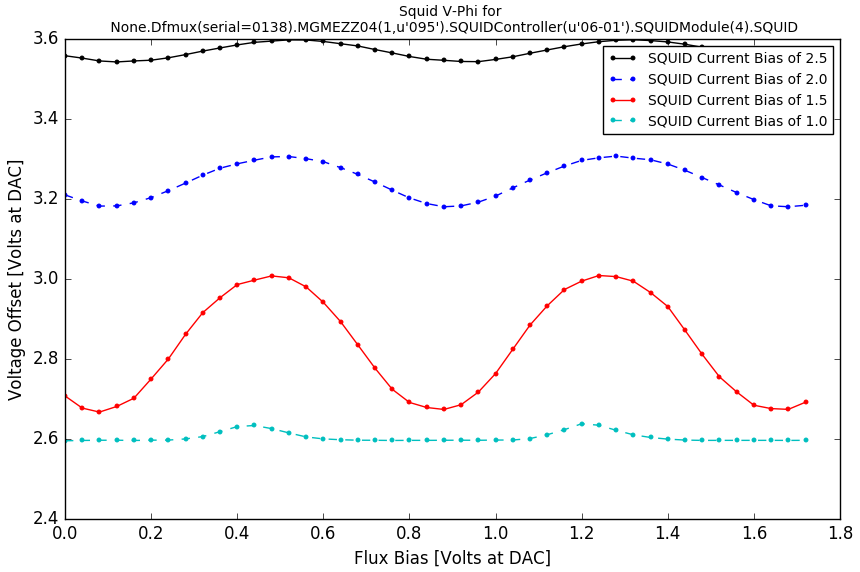
\includegraphics[width=\linewidth]{squid}
	\centering
	\caption{A voltage-flux curve produced by sweeping through flux biases for a range of SQUID bias currents, measuring the voltage required to zero the demodulated output.  The tuning algorithm correctly identifies the region of maximum gain and linearity in this case for a SQUID current bias of $\sim$1.6~A and flux bias of $\sim$0.7~V}
	\label{vphi}
\end{figure}

\begin{figure*}
	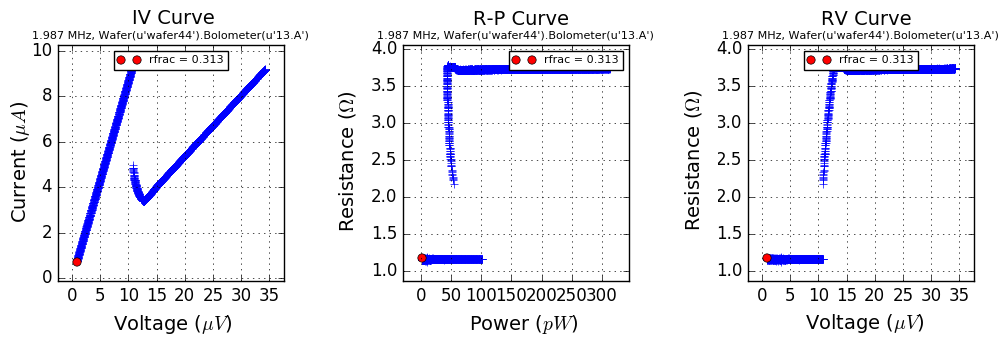
\includegraphics[width=\textwidth]{bolometer_bias}
	\centering
	\caption{Produced current-voltage (IV), resistance-power (RP), and resistance-voltage (RV) curves during the bolometer biasing process.  Bolometer `13.A' achieved a superconducting resistance 0.313 times that of its normal value.  The final state of the bolometer is shown in red.  The left figure demonstrates a linear decrease in current as the bias voltage is stepped down, with a turnaround into the superconducting region once the bias is sufficiently low.  The middle figure shows the saturation power on the bolometer island necessary for the bolometer to go superconducting, with a slight bend due to parasitic resistance located off the island.  Figure 3 demonstrates the sharp decrease in bolometer resistance as it transitions from its normal to superconducting state.}
	\label{bias}
\end{figure*}

The algorithm for tuning the SQUIDs to the region of maximum gain and linearity first starts by producing voltage-flux (V-Phi) curves for assorted SQUID current biases.  The flux bias Digital-to-Analog Converter (DAC) is sweeped through a range of values, mimicking the effect of a changing external magnetic field \citep{bender_digital_2014}.  The voltage required to zero the demodulated output is measured, forming a periodic function with peaks corresponding to 1/2 of the SQUID flux quanta.  The produced V-Phi curves for one of the SQUIDs is shown in Figure~\ref{vphi}, demonstrating the periodic voltage output as a function of flux quanta.  Following the V-Phi measurement, the tuning algorithm correctly identifies the SQUID current and flux bias for maximum gain, verifying SQUID performance.

\subsection{Network Analysis}

Once the SQUIDs have been successfully tuned, a network analysis algorithm works to identify each of the 64 $LCR_{bolo}$ resonant frequencies along with four additional resonances from calibration resistors.  The carrier and nuller DACs scan through a range of frequencies in the area of 200~kHz to 7~MHz, operating all 64 readout channels simultaneously until the full bandwidth of the system is probed.  The output demodulated amplitude is measured and averaged, producing the readout module response as a function of frequency.  A curve-fitting algorithm identifies each peak is the response, ideally producing 68 frequencies corresponding to each $LCR$ resonance.  

To account for systematics in the setup and allow for calibration, the installed configuration features two LC towers.  One services the wafer, while the other connects to a resistor board of known values and hence known resonances.  Early network analyses of the system produced poor results, with large noise levels causing the curve-fitting algorithm to fail.  Revisions to the cryostat grounding scheme (where ground loops can produce stray currents through electromagnetic induction) and RF environment were successful in reducing the noise level in the readout module response.  All 68 resonances were correctly identified, verifying this stage of the DfMUX readout system.   Each bolometer can now be targeted and biased through its unique resonant frequency.

\subsection{Bolometer Biasing}

The bolometer biasing operation starts by applying an AC bias voltage to each bolometer while above the superconducting transition temperature.  In this state, the bolometers behave like resistors and are referred to as being \textit{overbiased}.  The wafer temperature is then lowered below the transition temperature, but with the bias voltages holding each bolometer in its `normal' state.  Each bias voltage is then gradually stepped down, lowering the bolometers into their superconducting transition.  This process is demonstrated in Figure~\ref{bias}, clearly showing a linear decrease in measured current until a sufficiently low bias voltage is reached, at which point the bolometer transitions into its superconducting phase.  This be easily seen in the sharp drop in resistance between the normal and superconducting phases.

Following the successful bolometer biasing, information can be extracted on the critical TES temperatures, saturation power of the bolometers, and their normal/superconducting resistances.  This information is essential for feeding back into the wafer fabrication process, and even more so for the wafers that will be used in the deployment of \textsc{spt-3g}.  This also concludes the end-to-end verification of the developed \textsc{spt-3g} testing facility at UofT.

\section{\textsc{spt-pol} Data Processing}
\label{data_section}

\begin{figure*}
	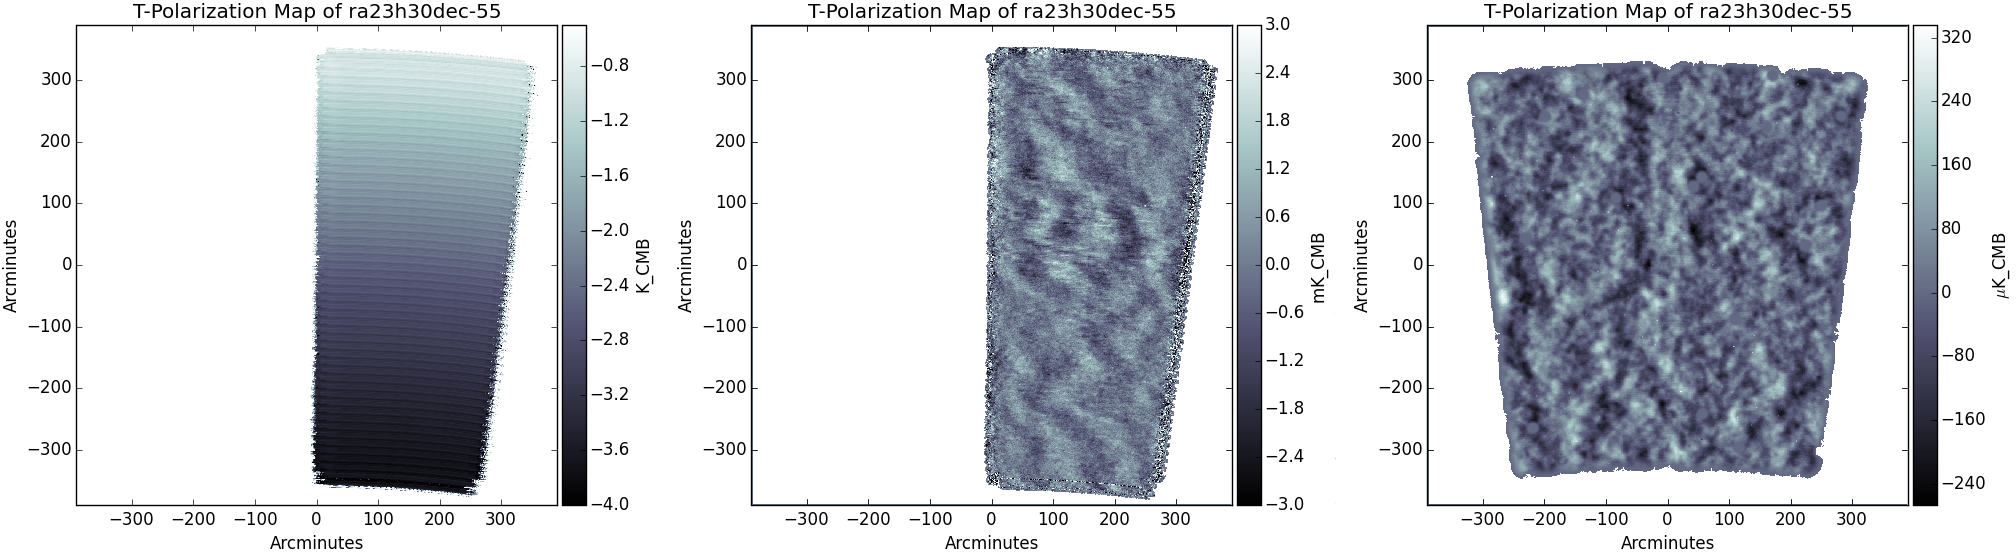
\includegraphics[width=\textwidth]{map_filtering}
	\centering
	\caption{Temperature maps produced using 150~GHz data from the \textsc{spt-pol} survey, looking at a 100 deg$^2$ squared patch of sky centred at RA 23$^h$30 and declination 55$^{\circ}$.  The left panel maps an unfiltered bolometer timestream, demonstrating the first order contamination effect of differing microwave temperature as a function of atmosphere thickness.  The middle panel shows the same timestream filtered with a fourth order polynomial and Gaussian smoothing profile, leaving small-scale atmospheric fluctuations. The right panel contains a full season's coaddition of filtered maps for the entire field, averaging out small-scale atmospheric fluctuations.  All that remains are the CMB temperature anisotropies.}
	\label{map}
\end{figure*}

The \textsc{spt-pol} survey was the polarization-sensitive survey by the SPT, looking at a 500 deg$^2$ patch of sky in the 90 and 150~GHz bands \citep{sptpol_2012}.  Many of the measurement, readout, and processing principals remain the same between this survey and \textsc{spt-3g}.  This section takes a brief look at the \textsc{spt-pol} processing used in converting bolometer timestreams into usable CMB maps and power spectra for extracting scientific data.

The raw telescope data is stored across multiple Hierarchical Data Format (HDF) databases, with each corresponding to a block of observation time.  Specific scans can be extracted from these databases, and stored as a minimally processed intermediate data file (IDF).  The developed \textit{SPTDataReader} allows the IDF files to be read in as python structures, allowing for easy access and manipulation of vast arrays of telescope data.  Including vital bolometer timestreams and scanning strategies, they even contain data such as wind speed and direction.

Figure~\ref{map} contains maps created using data from a 100 deg$^2$ survey centred at a Right Ascension (RA) of 23$^h$30 and Declination of 55$^{\circ}$.  The scanning strategy splits the field into two halves, using two identical raster scans in succession as the celestial sky rotates through the scanned region (scanning the whole field every hour).  The first panel in Figure~\ref{map} shows the mapped 150~GHz bolometer timestream from a single raster scan pattern, with minimal filtering to remove `bad' bolometers.  To the first order, all that can be seen is the difference in microwave temperature as a function of atmosphere thickness.  The middle panel in Figure~\ref{map} features the same mapped timestream, but using a fourth order polynomial fit to each scan segment along with a Gaussian smoothing profile.  The visible signal here is due to smaller-scale atmospheric fluctuations, which can be averaged out over multiple scans of the field.  The last panel in Figure~\ref{map} shows a coadded map of the entire field, averaged over scans taken throughout the course of an entire year (Feb. 2012 - Apr. 2013, excluding Austral summer).  Similar filtering is used to that of the middle panel, including point source removal and an apodization mask to smooth out the borders.

Once T, E, and B mode polarization maps have been  computed, the {spt-pol} software library contains a number of functions for producing their power spectra.  Map pairs can be used to create their cross-spectra, with options to mask specific features or vary the Fast Fourier Transform (FFT) shape.  As with the maps themselves, multiple map bundle pair's cross-spectra can be averaged, also producing the covariance between bins of the cross-spectrum.

\section{Conclusion}

I have presented here the development of a cryogenic testing environment for \textsc{spt-3g} at the University of Toronto.  Featuring a stable control system and web-interface, the HPD cryostat will assist in testing and characterizing \textsc{spt-3g} wafers and the DfMUX readout system.  Wafer characterization feedback is vital for the nanofabrication process currently underway at Argonne National Laboratory.  Each stage of the readout system from wafer to Iceboard has been installed and tested, allowing the TES bolometers on Wafer 44 to be successfully biased.  I have also presented maps and power spectra produced using \textsc{spt-pol} data, detailing the processing of bolometer current timestreams into usable scientific data from the CMB.  Once deployed, \textsc{spt-3g} will have appreciably advance the fields of large scale structure formation, particle physics, and cosmic inflation.



%\bibliography{biball2}
\begin{thebibliography}{dummy}
\bibitem[Addison et al.(2015)]{addison_quantifying_2015}
Addison, G. E., Huang, Y., Watts, D. J., et al. 2015, {arXiv:1511.00055 [astro-ph]}

\bibitem[Samtleben et al.(2007)]{samtleben_cosmic_2007}
Samtleben, D., Staggs, S., Winstein, B. 2007, in Annual Review of Nuclear and Particle Science, 245-283

\bibitem[Bender et al.(2014)]{bender_digital_2014}
Bender, A. N., Cliche, J. F., Haan, T., et al. 2014, {arXiv:1407.3161 [astro-ph]}

\bibitem[Henning et al.(2012)]{henning_feedhorn-coupled_2012}
Henning, J. W., Ade, P., Aird, K. A., et al. 2012, {arXiv:1210.4969 [astro-ph]}

\bibitem[Dobbs et al.(2012)]{dobbs_frequency_2012}
Dobbs, M. A., Lueker, M., Aird., K. A., et al. 2012, Review of Scientific Instruments, 83, 7

\bibitem[Benson et al.(2014)]{benson_spt-3g:_2014}
Benson, B. A., Ade, P. A. R., Ahmed, Z., et al. 2014, {arXiv:1407.2973 [astro-ph]}

\bibitem[Ruhl et al.(2004)]{spt_collaboration_south_2004}
Ruhl, J. E., Ade, P. A. R., Carlstrom, J. E., et al. 2004, {arXiv:astro-ph/0411122}

\bibitem[Posada et al.(2015)]{posada_fabrication_2015}
Posada, C. M., Ade, P. A. R., Ahmed, Z., et al. 2015, Superconductor Science and Technology, 28, 9

\bibitem[Austermann et al.(2012)]{sptpol_2012}
Austermann, J. E., Aird, K. A., Beall, J. A., et al. 2012, {arXiv:1210.4970 [astro-ph]}

\end{thebibliography}

\end{document}


